% Options for packages loaded elsewhere
\PassOptionsToPackage{unicode}{hyperref}
\PassOptionsToPackage{hyphens}{url}
\documentclass[
  english,
  10pt,
]{article}
\usepackage{xcolor}
\usepackage[margin=22mm]{geometry}
\usepackage{amsmath,amssymb}
\setcounter{secnumdepth}{-\maxdimen} % remove section numbering
\usepackage{iftex}
\ifPDFTeX
  \usepackage[T1]{fontenc}
  \usepackage[utf8]{inputenc}
  \usepackage{textcomp} % provide euro and other symbols
\else % if luatex or xetex
  \usepackage{unicode-math} % this also loads fontspec
  \defaultfontfeatures{Scale=MatchLowercase}
  \defaultfontfeatures[\rmfamily]{Ligatures=TeX,Scale=1}
\fi
\usepackage{lmodern}
\ifPDFTeX\else
  % xetex/luatex font selection
\fi
% Use upquote if available, for straight quotes in verbatim environments
\IfFileExists{upquote.sty}{\usepackage{upquote}}{}
\IfFileExists{microtype.sty}{% use microtype if available
  \usepackage[]{microtype}
  \UseMicrotypeSet[protrusion]{basicmath} % disable protrusion for tt fonts
}{}
\makeatletter
\@ifundefined{KOMAClassName}{% if non-KOMA class
  \IfFileExists{parskip.sty}{%
    \usepackage{parskip}
  }{% else
    \setlength{\parindent}{0pt}
    \setlength{\parskip}{6pt plus 2pt minus 1pt}}
}{% if KOMA class
  \KOMAoptions{parskip=half}}
\makeatother
\usepackage{color}
\usepackage{fancyvrb}
\newcommand{\VerbBar}{|}
\newcommand{\VERB}{\Verb[commandchars=\\\{\}]}
\DefineVerbatimEnvironment{Highlighting}{Verbatim}{commandchars=\\\{\}}
% Add ',fontsize=\small' for more characters per line
\newenvironment{Shaded}{}{}
\newcommand{\AlertTok}[1]{\textcolor[rgb]{1.00,0.00,0.00}{\textbf{#1}}}
\newcommand{\AnnotationTok}[1]{\textcolor[rgb]{0.38,0.63,0.69}{\textbf{\textit{#1}}}}
\newcommand{\AttributeTok}[1]{\textcolor[rgb]{0.49,0.56,0.16}{#1}}
\newcommand{\BaseNTok}[1]{\textcolor[rgb]{0.25,0.63,0.44}{#1}}
\newcommand{\BuiltInTok}[1]{\textcolor[rgb]{0.00,0.50,0.00}{#1}}
\newcommand{\CharTok}[1]{\textcolor[rgb]{0.25,0.44,0.63}{#1}}
\newcommand{\CommentTok}[1]{\textcolor[rgb]{0.38,0.63,0.69}{\textit{#1}}}
\newcommand{\CommentVarTok}[1]{\textcolor[rgb]{0.38,0.63,0.69}{\textbf{\textit{#1}}}}
\newcommand{\ConstantTok}[1]{\textcolor[rgb]{0.53,0.00,0.00}{#1}}
\newcommand{\ControlFlowTok}[1]{\textcolor[rgb]{0.00,0.44,0.13}{\textbf{#1}}}
\newcommand{\DataTypeTok}[1]{\textcolor[rgb]{0.56,0.13,0.00}{#1}}
\newcommand{\DecValTok}[1]{\textcolor[rgb]{0.25,0.63,0.44}{#1}}
\newcommand{\DocumentationTok}[1]{\textcolor[rgb]{0.73,0.13,0.13}{\textit{#1}}}
\newcommand{\ErrorTok}[1]{\textcolor[rgb]{1.00,0.00,0.00}{\textbf{#1}}}
\newcommand{\ExtensionTok}[1]{#1}
\newcommand{\FloatTok}[1]{\textcolor[rgb]{0.25,0.63,0.44}{#1}}
\newcommand{\FunctionTok}[1]{\textcolor[rgb]{0.02,0.16,0.49}{#1}}
\newcommand{\ImportTok}[1]{\textcolor[rgb]{0.00,0.50,0.00}{\textbf{#1}}}
\newcommand{\InformationTok}[1]{\textcolor[rgb]{0.38,0.63,0.69}{\textbf{\textit{#1}}}}
\newcommand{\KeywordTok}[1]{\textcolor[rgb]{0.00,0.44,0.13}{\textbf{#1}}}
\newcommand{\NormalTok}[1]{#1}
\newcommand{\OperatorTok}[1]{\textcolor[rgb]{0.40,0.40,0.40}{#1}}
\newcommand{\OtherTok}[1]{\textcolor[rgb]{0.00,0.44,0.13}{#1}}
\newcommand{\PreprocessorTok}[1]{\textcolor[rgb]{0.74,0.48,0.00}{#1}}
\newcommand{\RegionMarkerTok}[1]{#1}
\newcommand{\SpecialCharTok}[1]{\textcolor[rgb]{0.25,0.44,0.63}{#1}}
\newcommand{\SpecialStringTok}[1]{\textcolor[rgb]{0.73,0.40,0.53}{#1}}
\newcommand{\StringTok}[1]{\textcolor[rgb]{0.25,0.44,0.63}{#1}}
\newcommand{\VariableTok}[1]{\textcolor[rgb]{0.10,0.09,0.49}{#1}}
\newcommand{\VerbatimStringTok}[1]{\textcolor[rgb]{0.25,0.44,0.63}{#1}}
\newcommand{\WarningTok}[1]{\textcolor[rgb]{0.38,0.63,0.69}{\textbf{\textit{#1}}}}
\usepackage{longtable,booktabs,array}
\usepackage{calc} % for calculating minipage widths
% Correct order of tables after \paragraph or \subparagraph
\usepackage{etoolbox}
\makeatletter
\patchcmd\longtable{\par}{\if@noskipsec\mbox{}\fi\par}{}{}
\makeatother
% Allow footnotes in longtable head/foot
\IfFileExists{footnotehyper.sty}{\usepackage{footnotehyper}}{\usepackage{footnote}}
\makesavenoteenv{longtable}
\usepackage{graphicx}
\makeatletter
\newsavebox\pandoc@box
\newcommand*\pandocbounded[1]{% scales image to fit in text height/width
  \sbox\pandoc@box{#1}%
  \Gscale@div\@tempa{\textheight}{\dimexpr\ht\pandoc@box+\dp\pandoc@box\relax}%
  \Gscale@div\@tempb{\linewidth}{\wd\pandoc@box}%
  \ifdim\@tempb\p@<\@tempa\p@\let\@tempa\@tempb\fi% select the smaller of both
  \ifdim\@tempa\p@<\p@\scalebox{\@tempa}{\usebox\pandoc@box}%
  \else\usebox{\pandoc@box}%
  \fi%
}
% Set default figure placement to htbp
\def\fps@figure{htbp}
\makeatother
% definitions for citeproc citations
\NewDocumentCommand\citeproctext{}{}
\NewDocumentCommand\citeproc{mm}{%
  \begingroup\def\citeproctext{#2}\cite{#1}\endgroup}
\makeatletter
 % allow citations to break across lines
 \let\@cite@ofmt\@firstofone
 % avoid brackets around text for \cite:
 \def\@biblabel#1{}
 \def\@cite#1#2{{#1\if@tempswa , #2\fi}}
\makeatother
\newlength{\cslhangindent}
\setlength{\cslhangindent}{1.5em}
\newlength{\csllabelwidth}
\setlength{\csllabelwidth}{3em}
\newenvironment{CSLReferences}[2] % #1 hanging-indent, #2 entry-spacing
 {\begin{list}{}{%
  \setlength{\itemindent}{0pt}
  \setlength{\leftmargin}{0pt}
  \setlength{\parsep}{0pt}
  % turn on hanging indent if param 1 is 1
  \ifodd #1
   \setlength{\leftmargin}{\cslhangindent}
   \setlength{\itemindent}{-1\cslhangindent}
  \fi
  % set entry spacing
  \setlength{\itemsep}{#2\baselineskip}}}
 {\end{list}}
\usepackage{calc}
\newcommand{\CSLBlock}[1]{\hfill\break\parbox[t]{\linewidth}{\strut\ignorespaces#1\strut}}
\newcommand{\CSLLeftMargin}[1]{\parbox[t]{\csllabelwidth}{\strut#1\strut}}
\newcommand{\CSLRightInline}[1]{\parbox[t]{\linewidth - \csllabelwidth}{\strut#1\strut}}
\newcommand{\CSLIndent}[1]{\hspace{\cslhangindent}#1}
\ifLuaTeX
\usepackage[bidi=basic,shorthands=off,]{babel}
\else
\usepackage[bidi=default,shorthands=off,]{babel}
\fi
\ifLuaTeX
  \usepackage{selnolig} % disable illegal ligatures
\fi
\setlength{\emergencystretch}{3em} % prevent overfull lines
\providecommand{\tightlist}{%
  \setlength{\itemsep}{0pt}\setlength{\parskip}{0pt}}
\usepackage{etoolbox}
\AtBeginEnvironment{longtable}{\footnotesize}
\setlength{\tabcolsep}{4pt}
\usepackage{bookmark}
\IfFileExists{xurl.sty}{\usepackage{xurl}}{} % add URL line breaks if available
\urlstyle{same}
\hypersetup{
  pdftitle={Direct Source Supervision of Native Reconstruction Disagreement for Time-Series Anomaly Detection},
  pdflang={en},
  hidelinks,
  pdfcreator={LaTeX via pandoc}}

\title{Direct Source Supervision of Native Reconstruction Disagreement
for Time-Series Anomaly Detection}
\usepackage{etoolbox}
\makeatletter
\providecommand{\subtitle}[1]{% add subtitle to \maketitle
  \apptocmd{\@title}{\par {\large #1 \par}}{}{}
}
\makeatother
\subtitle{Research manuscript for assessment of methodological
contribution}
\author{}
\date{26 November 2026}

\begin{document}
\maketitle

\section{Abstract}\label{abstract}

A pretrained reconstruction detector may deploy disagreement among
masked reconstructions even when subsequent learning primarily rewards
reconstruction accuracy. We investigate direct supervision of that
deployed statistic. Starting from official TimeRadar weights, we freeze
the fractional representation and encoder and update only the native
decoder. Nominal source windows retain the per-copy reconstruction
objective. Publicly labeled abnormal and normal windows supply a
point-count-weighted pairwise loss on log-scaled endpoint variance.
Detection uses the same native variance with no additional head or
target parameter update. Three project-training seeds yield mean
average-precision gains over matched reconstruction continuation of
0.03433 on PSM, 0.01128 on MSL and 0.01665 on SMAP, while SMD decreases
by 0.00946. These seeds share one official initialization. Same-label
reconstruction-error and supervised-head comparisons support
task-dependent value for direct variance learning, with stronger
reconstruction-error performance on NASA and substantial gaps to
complete target-trained LEFT. Source-support expansion and full updates
fail to broaden competitiveness under the tested protocols. Operational
results expose false-alarm, event-discovery and coverage tradeoffs. The
evidence supports a narrowly defined source-supervised learning
procedure and identifies limits to its transfer.

\section{1 Introduction}\label{introduction}

Pretrained time-series anomaly detectors must convert internal outputs
into a scalar that ranks observations by abnormality. Reconstruction
error is one possible statistic. Disagreement across masked
reconstructions is another. Learning to reconstruct a nominal input and
learning to order abnormal observations by disagreement are related
objectives, but they need not favor the same parameters.

TimeRadar offers a concrete setting in which to examine this
distinction. Its official model learns an input-dependent fractional
representation and produces multiple masked reconstructions. The
released variance configuration measures disagreement among those copies
(He et al. 2026). A decoder can reduce reconstruction loss while
producing disagreement that transfers poorly as an anomaly score.
Deliberately increasing source-event disagreement could also separate
source examples yet damage target performance. Both possibilities
require detection evaluation.

We study a restricted intervention. We retain the official pretrained
representation, native decoder structure and endpoint variance. We
update the decoder with nominal reconstruction and a pairwise objective
applied directly to that variance on publicly labeled source events. The
endpoint supervised during fitting is also scored at deployment. The
method adds no scoring network. Five public SWaT fitting events and four
separate source-validation events supply anomaly knowledge. Nominal
reconstruction windows come from SWaT and SMD. Target parameters remain
frozen during the principal benchmark.

The technical question concerns the object being supervised. Pairwise
ranking, source anomaly labels, fractional transforms and reconstruction
variance have precedents. We examine one learning procedure in which
real source-event supervision changes the native deployment statistic
through the original decoder. This gives a precise implementation and
comparison. It also restricts the claim. The representation and
pretraining come from TimeRadar, and the experiments do not establish a
separate time--frequency representation contribution.

Three questions organize the study. Does direct endpoint-variance
supervision improve on frozen detection and source reconstruction
continuation under the same readout? How does the complete procedure
compare with reconstruction-error supervision, a standard supervised
head and mature external detectors? How stable are its gains across
source-training seeds, tasks and operating criteria?

The proposed contribution is the specification and implementation of
source-event supervision on native deployed endpoint disagreement, with
source-only checkpoint selection. The experimental contribution is a
matched three-seed evaluation and a set of same-label and
complete-method comparisons that locate the benefit and its boundaries.
These contributions concern a concrete learning procedure and its
observed transfer. Their significance is limited by inherited components
and by the evidence's scope.

The positive evidence consists of repeated average ranking gains on PSM
and two NASA tasks relative to the original reconstruction controls.
Important limitations remain. PSM informed development, SMD contributed
nominal source data, and NASA uses one sensor per entity. SMAP
precision--recall gains coexist with ROC costs. Complete LEFT is
stronger across most external comparisons. Completed mixed-update and
single-event-support experiments do not establish reliable additional
benefit.

\section{2 Related Work}\label{related-work}

\subsection{2.1 Pretrained detection and native
disagreement}\label{pretrained-detection-and-native-disagreement}

TimeRadar learns fractional reconstruction and contextual deviation in
hidden patches. Its published detection rule includes reconstruction
error and variability among masked outputs (He et al. 2026). We
distinguish that combined rule from the fixed released-code variance
configuration used here. Our intervention supervises the native endpoint
variance after official pretraining.

DADA combines an adaptive bottleneck with dual adversarial decoders and
also uses reconstruction variability for detection (Shentu et al. 2025).
Variance-based anomaly evidence is therefore established prior work.
TimeRCD learns a contextual anomaly discriminator using synthetic
context-dependent labels (Lan et al. 2026). Our procedure applies real
public source labels to the original TimeRadar decoder and keeps its
variance readout. Complete comparisons assess competitive scope. Matched
TimeRadar controls provide the closer evidence for the training
intervention.

\subsection{2.2 Source supervision and pairwise
learning}\label{source-supervision-and-pairwise-learning}

Neural pairwise ranking is a mature tool (Burges et al. 2005). Learning
anomaly scores from limited labels also precedes this work. PReNet
learns relations between labeled and unlabeled instances to obtain
anomaly scores (Pang et al. 2019). We use a softplus margin on two
native scalar scores. The object differentiated through is an existing
reconstruction-disagreement statistic, alongside nominal reconstruction.

Source labels identify full abnormal or normal windows. They do not
identify individual faulty sensors. Three chronological endpoint strata
support sampling within each event, with weights proportional to their
legal positive endpoint counts. These strata provide no physical stage
interpretation. Source and target datasets also have different anomaly
semantics.

\subsection{2.3 Multiview detectors and information
permissions}\label{multiview-detectors-and-information-permissions}

LEFT coordinates temporal, spectral and multiscale views through
reconstruction and consistency objectives (Wang et al. 2026). CATCH
models channel relationships using frequency patching (Wu et al. 2025).
We retain their complete local implementations as external references
where compatible caches exist.

A common timestamp axis aligns evaluated observations but leaves
information differences intact. Interior scores from a full window
become available after the scored observation. A terminal score uses the
current observation and preceding window. Our causal ranking and
external common-axis panels therefore retain their respective
availability times and standardization permissions. Global ranking,
empirical false alarms and event discovery are reported as distinct
outcomes.

\section{3 Problem Formulation}\label{problem-formulation}

Let a public record contain \(x_0,\ldots,x_{N-1}\), with
\(x_t\in\mathbb R^C\). An archived scaler fitted on permitted nominal
FIT data gives \(z_t\). An eligible timestamp has input \[
X_t=[z_{t-99},\ldots,z_t]\in\mathbb R^{100\times C}.
\] Each native forward contains one window. The current observation
participates in reconstruction. The endpoint score is available at
\(t\).

Sources supply nominal windows \(\mathcal N\), labeled fitting events
\(\mathcal E_{\rm fit}\), and separate labeled selection events
\(\mathcal E_{\rm select}\). A positive window lies entirely inside an
abnormal source interval. Its paired negative lies entirely inside a
labeled-normal interval of the same authorized role. Source labels enter
fitting and checkpoint selection.

Each target has a fixed scoring axis \(\mathcal I_d\). Target labels
enter evaluation after source selection. Target parameters receive zero
updates. Archived target FIT values may supply scaler statistics. CAL
values determine empirical thresholds for the separate operating
analysis. The official checkpoint's upstream pretraining permissions are
inherited, and exclusion of every target dataset from all upstream
pretraining is not independently certified.

AP is the principal outcome. ROC-AUC, VUS-PR and VUS-ROC complement it.
For multi-entity tasks we compute metrics per entity, then take
equal-weight means. Three seeds vary project source sampling and fitting
from one official initialization. They are not independent datasets or
independent pretrained models.

\section{4 Proposed Method}\label{proposed-method}

\subsection{4.1 Frozen representation and native
decoder}\label{frozen-representation-and-native-decoder}

Write the official forward as \[
H^{(m)}(X;\theta_0,\mathcal M_C),\qquad
\widehat X_\psi^{(m)}
=\left|\operatorname{iFRFT}_{\alpha_{\theta_0}(X)}
\!\left(D_\psi(H^{(m)})\right)\right|,
\quad m=1,\ldots, 10.
\] The fixed parameters \(\theta_0\) include the order network,
real/imaginary input mappings and encoder. \(D_\psi\) is the original
complex decoder. The order is computed independently for each B=1 window
using its variables according to the native rule. Official fractional
transforms and variable ordering are retained.

The mask bank \(\mathcal M_C\) contains five fixed random patch masks
and their complements. RNG state is isolated and restored around each
forward. Masks depend on channel count and are fixed across fitting and
scoring. Eval mode disables dropout while decoder gradients remain
enabled. All non-decoder parameters and buffers are frozen.

\begin{figure}
\centering
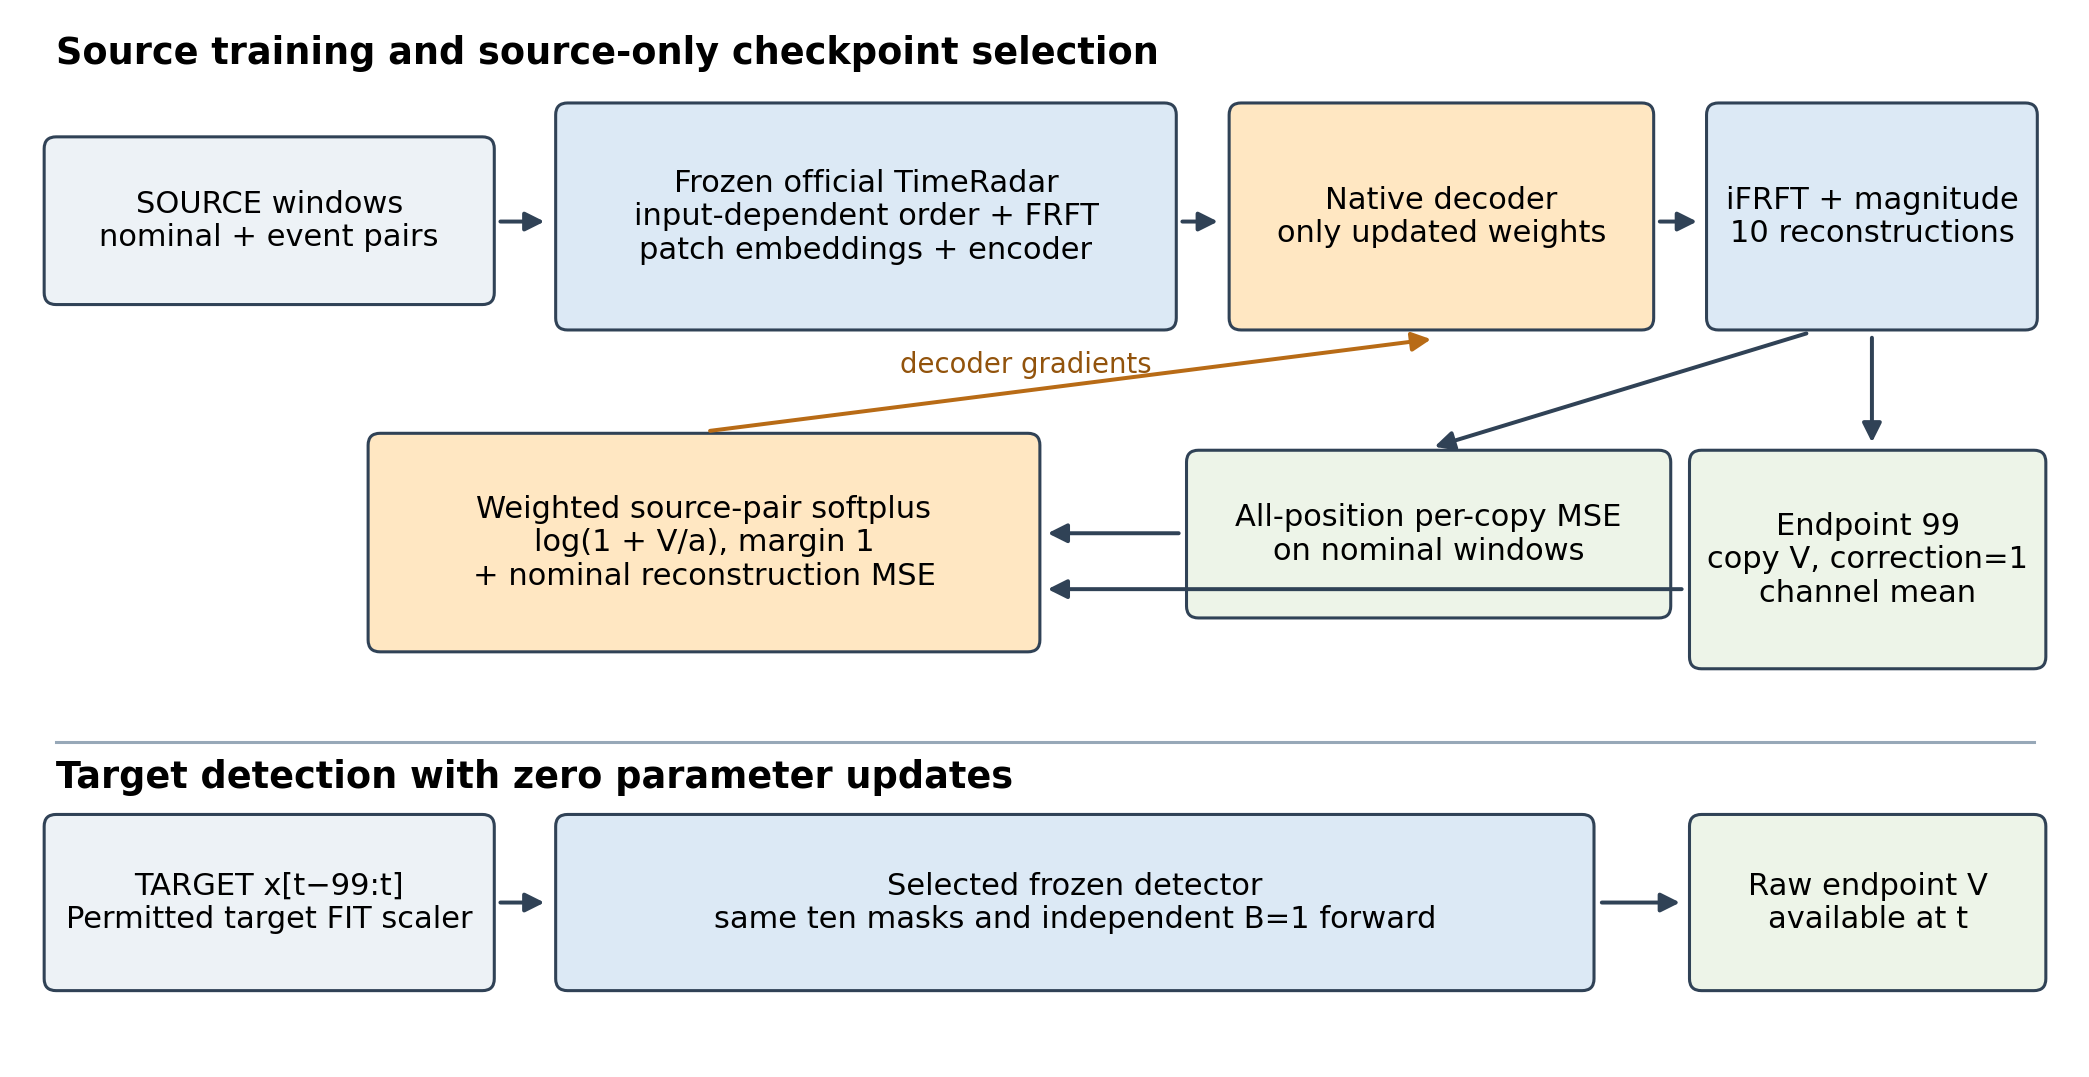
\includegraphics[width=1\linewidth,height=\textheight,keepaspectratio,alt={The single formal method. Source learning changes only the native decoder. Nominal reconstruction uses all positions, whereas pair supervision and deployment use endpoint 99. Each target window has its own native B=1 forward.}]{figures/method.png}
\caption{The single formal method. Source learning changes only the
native decoder. Nominal reconstruction uses all positions, whereas pair
supervision and deployment use endpoint 99. Each target window has its
own native B=1 forward.}
\end{figure}

\subsection{4.2 Deployment statistic and nominal
objective}\label{deployment-statistic-and-nominal-objective}

Define the copy mean \[
\overline x_{\psi,j,c}=\frac 1{10}\sum_{m=1}^{10}\widehat X_{\psi,j,c}^{(m)}.
\] The deployment statistic is \[
V_\psi(X)=\frac 1C\sum_{c=1}^{C}\frac 1{9}
\sum_{m=1}^{10}
\left(\widehat X_{\psi, 99,c}^{(m)}
-\overline x_{\psi, 99,c}\right)^2.
\tag{1}
\] This uses correction 1 and the channel mean. Ten copies and position
99 are identical in the training pairs and deployment.

Nominal windows retain the complete per-copy objective \[
\mathcal L_{\rm copy}=
\frac 1{|\mathcal B_N|}\sum_{X\in\mathcal B_N}
\frac 1{10\cdot 100\cdot C_X}
\sum_{m,j,c}
\left(\widehat X_{\psi,j,c}^{(m)}-X_{j,c}\right)^2.
\tag{2}
\] Each window is reduced before averaging, so sources with different
channel counts receive equal weight per window.

This loss decomposes exactly into \[
\mathcal L_{\rm copy}(X)=E_{\rm full}(X)+0.9V_{\rm full}(X),
\] where both terms average all positions and channels, and the variance
uses correction 1. Nominal reconstruction therefore already penalizes
disagreement on nominal windows. It supplies no direct ordering
constraint between labeled abnormal and normal endpoints. That
distinction motivates supervision, without identifying a unique cause of
historical failures.

\subsection{4.3 Weighted endpoint pair
learning}\label{weighted-endpoint-pair-learning}

Partition each fitting event's legal endpoints into three chronological,
nearly equal-size strata \(\mathcal P_{e,k}\). Let
\(n_{e,k}=|\mathcal P_{e,k}|\). Each update samples one positive window
\(P_{e,k}\) per stratum and one negative \(N_{e,k}\) from the legal
labeled-normal pool. Set \[
w_{e,k}=\frac{n_{e,k}}{\sum_{e',k'}n_{e',k'}},
\qquad
g_\psi(X)=\log\!\left(1+\frac{V_\psi(X)}a\right).
\] The fixed \(a\) is the official-initialization median V over all
4,632 legal normal source-FIT endpoints, protected below by \(10^{-8}\).
Its archived value is \(0.02649214304983616\).

The supervised and total losses are \[
\mathcal L_{\rm pair}
=\sum_{e,k}w_{e,k}\operatorname{softplus}
\!\left(1-g_\psi(P_{e,k})+g_\psi(N_{e,k})\right),
\tag{3}
\] \[
\mathcal L=\mathcal L_{\rm copy}+\mathcal L_{\rm pair}.
\tag{4}
\] Margin and pair coefficient are both 1. The weights describe
window-sampling strata. Overlapping windows do not become independent
events or uniformly supervised original timepoints.

For \(u=1-g(P)+g(N)\), \[
\frac{\partial\ell}{\partial V(P)}
=-\frac{\sigma(u)}{a+V(P)},\qquad
\frac{\partial\ell}{\partial V(N)}
=\frac{\sigma(u)}{a+V(N)}.
\tag{5}
\] The objective encourages positive source disagreement relative to its
paired negative through the decoder. Nominal reconstruction provides the
accompanying constraint. These derivative directions describe the
learning request. They imply no transfer guarantee for new events or
domains.

Updating only \(\psi\) preserves upstream parameters while permitting
the decoder to alter the relation between features and reconstructed
copies. Variance can change independently of whether an input is
accurately reconstructed. We therefore evaluate direct E supervision and
a supervised head as separate complete procedures.

\subsection{4.4 Source selection and
implementation}\label{source-selection-and-implementation}

The five fitting events yield 15 strata. Each update uses 32 nominal
windows, 16 SWaT and 16 SMD, plus 15 positive and 15 paired-normal
windows. SMD first samples a machine uniformly, then a legal endpoint.
Independent native B=1 forwards accumulate decoder gradients before one
optimizer step.

Fresh AdamW uses learning rate \(10^{-4}\), betas \((0.9,0.95)\),
epsilon \(10^{-8}\), weight decay 0.1 excluding bias and LayerNorm
parameters, and 24-step linear warmup. The cap is 240 updates. At
updates \(0,40,\ldots, 240\), source selection evaluates 16 fixed pairs
per validation event/stratum. Risk averages pairs within each stratum,
then equally over four events and three strata. The earliest minimum
wins. Training is point-count weighted and selection is event/stratum
balanced. The reconstruction control uses this same label-assisted
selection. Selected steps and exposures differ across methods.

\textbf{Algorithm 1. Direct source supervision of native endpoint V}

\begin{Shaded}
\begin{Highlighting}[]
\NormalTok{Inputs: official parameters (theta 0, psi 0), fixed source roles,}
\NormalTok{        seed{-}specific window plan, mask bank M\_C, source scale a}
\NormalTok{Freeze theta \textless{}{-} theta 0; set trainable psi \textless{}{-} psi 0}
\NormalTok{Keep the complete model in eval mode; create fresh decoder AdamW}
\NormalTok{best\_risk \textless{}{-} infinity}
\NormalTok{For q = 0,...,240}
\NormalTok{    If q \textgreater{} 0}
\NormalTok{        Clear decoder gradients}
\NormalTok{        For each of the 32 nominal windows X in plan[q]}
\NormalTok{            Native B=1 forward with isolated fixed masks}
\NormalTok{            Backpropagate copy\_MSE(X)/32}
\NormalTok{        Draw one positive and one normal window for each FIT stratum}
\NormalTok{        Native B=1 forward for each paired window}
\NormalTok{        Compute V at endpoint 99 and weighted pair loss (Equation 3)}
\NormalTok{        Backpropagate pair loss}
\NormalTok{        Apply scheduled learning rate and one AdamW step}
\NormalTok{    If q in \{0,40,80,120,160,200,240\}}
\NormalTok{        Compute the fixed SOURCE SELECT event/stratum risk}
\NormalTok{        If risk \textless{} best\_risk, save decoder and update best\_risk}
\NormalTok{Freeze the selected decoder}
\NormalTok{For each legal target timestamp t}
\NormalTok{    Apply the permitted archived target scaler}
\NormalTok{    Form X\_t = z[t{-}99:t+1]; native B=1 forward with fixed masks}
\NormalTok{    Output raw V(X\_t); available\_index \textless{}{-} t}
\end{Highlighting}
\end{Shaded}

The implementation is in native\_event\_rank.py,
native\_event\_rank\_training.py and the archived domain readouts.
Native score computation retains decoder gradients through the inverse
transform. The training score uses cal\_anomaly\_score with L=1. Source
selection precedes target scoring.

\section{5 Experiments}\label{experiments}

\subsection{5.1 Public data and axes}\label{public-data-and-axes}

PSM uses 25 channels and SMD all 28 machines with 38 channels. NASA uses
sensor column 0 for 27 MSL and 53 admitted SMAP entities. The archived
admission rule excludes SMAP P-2 because of a pre-existing label/record
conflict. The rule predates these comparisons. Complete causal axes are
\([99,N)\) within records, totaling 87,742 PSM, 705,648 SMD, 71,056 MSL
and 422,370 SMAP points. Entities are never concatenated into a
continuous record.

Nominal SWaT FIT is \([0,396000)\). The authorized labeled slice
\([495000,585000)\) splits at 502578, in a normal inter-event gap. Five
fitting events provide 1,857 legal positive endpoints and 4,632 legal
normal endpoints. Four selection events provide 2,439 positive and
79,092 normal endpoints. SWaT is excluded as a target for this fold. SMD
nominal training-side FIT supplies reconstruction windows.

PSM is exposed development data. SMD evaluates held-out tests of
nominal-source-visible devices. NASA supplies different public tasks
with single-sensor inputs. These permissions differ from fully
unseen-domain testing. Target FIT scalers are retained from the archived
protocol.

The external common axis starts at 99 and ends at each entity's last
point jointly scored by LEFT and DADA. Totals are 87,645 PSM, 702,996
SMD, 69,495 MSL and 417,265 SMAP points. Our causal values are
restricted to those indices without changing their scores. LEFT uses W96
on MSL and W192 elsewhere, DADA W100, and TimeRCD blocks up to 5000
points. Their interior scores retain later availability. A separate
history-baseline panel appears in the supplement.

\subsection{5.2 Metrics and comparisons}\label{metrics-and-comparisons}

AP is non-interpolated average precision, distinct from trapezoidal PR
area. ROC-AUC and both VUS metrics accompany it. VUS uses the pinned
LEFT implementation with windowSize 100 and 250 thresholds. It
incorporates tolerance around ranges and is interpreted alongside strict
point ranking.

Frozen official V, E and V+E are local project endpoint results. Here \[
E_\psi(X)=\frac 1C\sum_c
(\overline x_{\psi, 99,c}-X_{99,c})^2.
\] The fixed sum is the existing paper-formula comparison under the
project endpoint protocol. It is separate from released-code L=1 V and
from exact reproduction of the author's complete original evaluation
track.

Source reconstruction uses the original nominal draws and labeled
SELECT. Direct E shares the labeled pair schedule and loss form but uses
its own official-normal FIT scale 0.30042700469493866 and E-specific
selection risk. The MLP uses frozen official features with a supervised
nonlinear readout. It changes trainable components, objective and score,
so it is a complete supervised control.

LEFT trains on target nominal arrays with normal validation. SMD has
per-machine models and NASA domain-shared models. Its scaler includes
the complete normal prefix. DADA uses official weights and normal target
arrays for scaling. TimeRCD uses official logit differences with
archived FIT-only statistics once. NASA uses its official univariate
checkpoint. Whole-QUERY statistics remain in their separate archived
track. CATCH and PCA retain their existing target-training permissions.

Seeds 2025--2027 vary source sampling from one pretrained initial state.
We report sample SD with ddof 1. Paired differences are computed at each
seed before averaging. Entity count and overlapping point count do not
enlarge the number of training repetitions. No significance claim is
made from three seeds.

\subsection{5.3 Complete detectors}\label{complete-detectors}

Table 1 uses the external common axis. Cells contain two metrics each.
Trained native controls show three-seed mean and sample SD. Single
official/external results retain their fixed identity. Every value is a
local computation, including project protocol adaptations.

\textbf{Table 1A. Complete methods, AP / ROC-AUC.}

\begin{longtable}[]{@{}
  >{\raggedright\arraybackslash}p{(\linewidth - 8\tabcolsep) * \real{0.2000}}
  >{\raggedright\arraybackslash}p{(\linewidth - 8\tabcolsep) * \real{0.2000}}
  >{\raggedright\arraybackslash}p{(\linewidth - 8\tabcolsep) * \real{0.2000}}
  >{\raggedright\arraybackslash}p{(\linewidth - 8\tabcolsep) * \real{0.2000}}
  >{\raggedright\arraybackslash}p{(\linewidth - 8\tabcolsep) * \real{0.2000}}@{}}
\toprule\noalign{}
\begin{minipage}[b]{\linewidth}\raggedright
Method
\end{minipage} & \begin{minipage}[b]{\linewidth}\raggedright
PSM
\end{minipage} & \begin{minipage}[b]{\linewidth}\raggedright
SMD28
\end{minipage} & \begin{minipage}[b]{\linewidth}\raggedright
MSL27
\end{minipage} & \begin{minipage}[b]{\linewidth}\raggedright
SMAP53
\end{minipage} \\
\midrule\noalign{}
\endhead
\bottomrule\noalign{}
\endlastfoot
Frozen TimeRadar V & 0.5353 / 0.7310 & 0.4448 / 0.8132 & 0.3426 / 0.6327
& 0.3656 / 0.6427 \\
Frozen TimeRadar E & 0.3873 / 0.5697 & 0.4291 / 0.8053 & 0.3904 / 0.6932
& 0.4254 / 0.6805 \\
Frozen fixed V + E & 0.4195 / 0.6034 & 0.4388 / 0.8121 & 0.3999 / 0.7037
& 0.4148 / 0.7080 \\
Source reconstruction (3 seeds) & 0.5388 ± 0.0021 / 0.7317 ± 0.0009 &
0.4497 ± 0.0026 / 0.8187 ± 0.0037 & 0.3494 ± 0.0019 / 0.6363 ± 0.0016 &
0.3663 ± 0.0022 / 0.6359 ± 0.0042 \\
Direct V (3 seeds) & 0.5731 ± 0.0047 / 0.7640 ± 0.0028 & 0.4402 ± 0.0025
/ 0.8261 ± 0.0011 & 0.3659 ± 0.0019 / 0.6678 ± 0.0030 & 0.3826 ± 0.0022
/ 0.6317 ± 0.0047 \\
Complete LEFT (1 seed) & 0.5769 / 0.7762 & 0.4981 / 0.8785 & 0.5083 /
0.7633 & 0.4932 / 0.7629 \\
Complete DADA & 0.3957 / 0.6050 & 0.4146 / 0.8514 & 0.3957 / 0.7336 &
0.4288 / 0.6459 \\
TimeRCD, FIT-only & 0.3019 / 0.4762 & 0.4729 / 0.8594 & 0.4827 / 0.7631
& 0.4427 / 0.6749 \\
CATCH seed0 & 0.4465 / 0.6538 & NA & NA & NA \\
CATCH seed1 & 0.4307 / 0.6417 & NA & NA & NA \\
CATCH seed2 & 0.4334 / 0.6475 & NA & NA & NA \\
PCA & 0.5344 / 0.7931 & NA & NA & NA \\
\end{longtable}

\textbf{Table 1B. Identical methods and axes, VUS-PR / VUS-ROC.}

\begin{longtable}[]{@{}
  >{\raggedright\arraybackslash}p{(\linewidth - 8\tabcolsep) * \real{0.2000}}
  >{\raggedright\arraybackslash}p{(\linewidth - 8\tabcolsep) * \real{0.2000}}
  >{\raggedright\arraybackslash}p{(\linewidth - 8\tabcolsep) * \real{0.2000}}
  >{\raggedright\arraybackslash}p{(\linewidth - 8\tabcolsep) * \real{0.2000}}
  >{\raggedright\arraybackslash}p{(\linewidth - 8\tabcolsep) * \real{0.2000}}@{}}
\toprule\noalign{}
\begin{minipage}[b]{\linewidth}\raggedright
Method
\end{minipage} & \begin{minipage}[b]{\linewidth}\raggedright
PSM
\end{minipage} & \begin{minipage}[b]{\linewidth}\raggedright
SMD28
\end{minipage} & \begin{minipage}[b]{\linewidth}\raggedright
MSL27
\end{minipage} & \begin{minipage}[b]{\linewidth}\raggedright
SMAP53
\end{minipage} \\
\midrule\noalign{}
\endhead
\bottomrule\noalign{}
\endlastfoot
Frozen TimeRadar V & 0.4836 / 0.6648 & 0.4672 / 0.8700 & 0.4147 / 0.7048
& 0.4027 / 0.6902 \\
Frozen TimeRadar E & 0.3985 / 0.5814 & 0.4336 / 0.8487 & 0.4701 / 0.7671
& 0.4686 / 0.7386 \\
Frozen fixed V + E & 0.4237 / 0.6074 & 0.4428 / 0.8552 & 0.4805 / 0.7739
& 0.4558 / 0.7594 \\
Source reconstruction (3 seeds) & 0.4901 ± 0.0052 / 0.6664 ± 0.0020 &
0.4749 ± 0.0046 / 0.8741 ± 0.0027 & 0.4229 ± 0.0019 / 0.7076 ± 0.0016 &
0.3977 ± 0.0024 / 0.6790 ± 0.0017 \\
Direct V (3 seeds) & 0.5084 ± 0.0049 / 0.6757 ± 0.0039 & 0.4300 ± 0.0054
/ 0.8598 ± 0.0015 & 0.4345 ± 0.0028 / 0.7356 ± 0.0050 & 0.4300 ± 0.0033
/ 0.6819 ± 0.0046 \\
Complete LEFT (1 seed) & 0.5741 / 0.7858 & 0.5418 / 0.9185 & 0.5531 /
0.7942 & 0.5217 / 0.7849 \\
Complete DADA & 0.4395 / 0.6520 & 0.4747 / 0.8997 & 0.4298 / 0.7747 &
0.4459 / 0.6826 \\
TimeRCD, FIT-only & 0.3485 / 0.5320 & 0.5151 / 0.9098 & 0.5298 / 0.8065
& 0.4280 / 0.7038 \\
CATCH seed0 & 0.5361 / 0.7028 & NA & NA & NA \\
CATCH seed1 & 0.5187 / 0.6898 & NA & NA & NA \\
CATCH seed2 & 0.5267 / 0.6983 & NA & NA & NA \\
PCA & 0.5287 / 0.7670 & NA & NA & NA \\
\end{longtable}

The candidate's strongest competitive scope is PSM. Its mean AP0.5731 is
close to LEFT0.5769 and above DADA0.3957 and FIT-only TimeRCD0.3019.
LEFT has higher ROC and both VUS measures. SMD candidate AP0.4402 is
below LEFT and TimeRCD and above DADA. Its mean margin over DADA
includes negative entity medians and only 12--13 winning machines across
seeds.

NASA exposes larger gaps. Candidate mean AP is 0.3659 on MSL and 0.3826
on SMAP, compared with LEFT0.5083 and 0.4932. DADA and TimeRCD also have
higher AP. Frozen E and V+E remain strong NASA references. These limits
coexist with gains over matched native controls.

\subsection{5.4 Repeated learning
effects}\label{repeated-learning-effects}

Table 2 reports method means and seed SDs on complete causal axes. Table
3 reports within-seed differences and their SDs. Difference uncertainty
must be calculated from paired values.

\textbf{Table 2. Complete causal axes, method values.}

\begin{longtable}[]{@{}
  >{\raggedright\arraybackslash}p{(\linewidth - 12\tabcolsep) * \real{0.1429}}
  >{\raggedright\arraybackslash}p{(\linewidth - 12\tabcolsep) * \real{0.1429}}
  >{\raggedright\arraybackslash}p{(\linewidth - 12\tabcolsep) * \real{0.1429}}
  >{\raggedright\arraybackslash}p{(\linewidth - 12\tabcolsep) * \real{0.1429}}
  >{\raggedright\arraybackslash}p{(\linewidth - 12\tabcolsep) * \real{0.1429}}
  >{\raggedright\arraybackslash}p{(\linewidth - 12\tabcolsep) * \real{0.1429}}
  >{\raggedright\arraybackslash}p{(\linewidth - 12\tabcolsep) * \real{0.1429}}@{}}
\toprule\noalign{}
\begin{minipage}[b]{\linewidth}\raggedright
Domain
\end{minipage} & \begin{minipage}[b]{\linewidth}\raggedright
Method
\end{minipage} & \begin{minipage}[b]{\linewidth}\raggedright
Training seeds
\end{minipage} & \begin{minipage}[b]{\linewidth}\raggedright
AP
\end{minipage} & \begin{minipage}[b]{\linewidth}\raggedright
ROC\_AUC
\end{minipage} & \begin{minipage}[b]{\linewidth}\raggedright
VUS\_PR
\end{minipage} & \begin{minipage}[b]{\linewidth}\raggedright
VUS\_ROC
\end{minipage} \\
\midrule\noalign{}
\endhead
\bottomrule\noalign{}
\endlastfoot
PSM & Frozen V & 1 & 0.53521 & 0.73065 & 0.48391 & 0.66457 \\
PSM & Reconstruction & 3 & 0.53874 ± 0.00208 & 0.73136 ± 0.00094 &
0.49047 ± 0.00519 & 0.66623 ± 0.00197 \\
PSM & Direct V & 3 & 0.57307 ± 0.00467 & 0.76382 ± 0.00275 & 0.50889 ±
0.00487 & 0.67571 ± 0.00386 \\
SMD & Frozen V & 1 & 0.44423 & 0.81295 & 0.46636 & 0.86971 \\
SMD & Reconstruction & 3 & 0.44909 ± 0.00258 & 0.81849 ± 0.00365 &
0.47381 ± 0.00443 & 0.87381 ± 0.00271 \\
SMD & Direct V & 3 & 0.43963 ± 0.00254 & 0.82581 ± 0.00108 & 0.42868 ±
0.00545 & 0.85949 ± 0.00150 \\
MSL & Frozen V & 1 & 0.33559 & 0.62874 & 0.40570 & 0.70148 \\
MSL & Reconstruction & 3 & 0.34139 ± 0.00138 & 0.63255 ± 0.00164 &
0.41301 ± 0.00162 & 0.70444 ± 0.00166 \\
MSL & Direct V & 3 & 0.35267 ± 0.00162 & 0.66251 ± 0.00281 & 0.42019 ±
0.00249 & 0.73057 ± 0.00468 \\
SMAP & Frozen V & 1 & 0.36560 & 0.64193 & 0.40267 & 0.68870 \\
SMAP & Reconstruction & 3 & 0.36623 ± 0.00213 & 0.63499 ± 0.00417 &
0.39735 ± 0.00220 & 0.67737 ± 0.00170 \\
SMAP & Direct V & 3 & 0.38287 ± 0.00213 & 0.63104 ± 0.00462 & 0.42961 ±
0.00357 & 0.68028 ± 0.00497 \\
\end{longtable}

\textbf{Table 3. Same-axis paired differences, mean ± sample SD, n=3.}

\begin{longtable}[]{@{}
  >{\raggedright\arraybackslash}p{(\linewidth - 10\tabcolsep) * \real{0.1667}}
  >{\raggedright\arraybackslash}p{(\linewidth - 10\tabcolsep) * \real{0.1667}}
  >{\raggedright\arraybackslash}p{(\linewidth - 10\tabcolsep) * \real{0.1667}}
  >{\raggedright\arraybackslash}p{(\linewidth - 10\tabcolsep) * \real{0.1667}}
  >{\raggedright\arraybackslash}p{(\linewidth - 10\tabcolsep) * \real{0.1667}}
  >{\raggedright\arraybackslash}p{(\linewidth - 10\tabcolsep) * \real{0.1667}}@{}}
\toprule\noalign{}
\begin{minipage}[b]{\linewidth}\raggedright
Domain
\end{minipage} & \begin{minipage}[b]{\linewidth}\raggedright
Within-seed contrast
\end{minipage} & \begin{minipage}[b]{\linewidth}\raggedright
AP
\end{minipage} & \begin{minipage}[b]{\linewidth}\raggedright
ROC\_AUC
\end{minipage} & \begin{minipage}[b]{\linewidth}\raggedright
VUS\_PR
\end{minipage} & \begin{minipage}[b]{\linewidth}\raggedright
VUS\_ROC
\end{minipage} \\
\midrule\noalign{}
\endhead
\bottomrule\noalign{}
\endlastfoot
PSM & Direct V − frozen V & +0.03786 ± 0.00467 & +0.03317 ± 0.00275 &
+0.02497 ± 0.00487 & +0.01115 ± 0.00386 \\
PSM & Direct V − reconstruction & +0.03433 ± 0.00343 & +0.03246 ±
0.00199 & +0.01841 ± 0.00408 & +0.00948 ± 0.00328 \\
SMD & Direct V − frozen V & -0.00460 ± 0.00254 & +0.01286 ± 0.00108 &
-0.03767 ± 0.00545 & -0.01022 ± 0.00150 \\
SMD & Direct V − reconstruction & -0.00946 ± 0.00397 & +0.00732 ±
0.00324 & -0.04513 ± 0.00778 & -0.01432 ± 0.00323 \\
MSL & Direct V − frozen V & +0.01707 ± 0.00162 & +0.03377 ± 0.00281 &
+0.01449 ± 0.00249 & +0.02909 ± 0.00468 \\
MSL & Direct V − reconstruction & +0.01128 ± 0.00119 & +0.02996 ±
0.00359 & +0.00718 ± 0.00186 & +0.02613 ± 0.00530 \\
SMAP & Direct V − frozen V & +0.01727 ± 0.00213 & -0.01089 ± 0.00462 &
+0.02694 ± 0.00357 & -0.00842 ± 0.00497 \\
SMAP & Direct V − reconstruction & +0.01665 ± 0.00217 & -0.00395 ±
0.00710 & +0.03226 ± 0.00572 & +0.00291 ± 0.00556 \\
\end{longtable}

Direct V improves AP over both controls at every seed on PSM, MSL and
SMAP. PSM and MSL also improve both ROC and VUS measures. SMAP improves
AP and VUS-PR but reduces ROC-AUC against frozen V in every seed. SMD
loses AP and both VUS measures with a higher ROC-AUC. The fixed endpoint
intervention produces repeatable yet task-dependent changes.

Against reconstruction, MSL has 16--17 AP wins among 27 entities. SMAP
has 28--30 among 53, with small positive medians. Against frozen V, SMAP
medians are near zero and win counts vary. The supplement retains all
per-seed distributions. The number of target points does not increase
the training repeat count.

\subsection{5.5 Training statistic and supervised
readout}\label{training-statistic-and-supervised-readout}

Table 4 uses seed 2025 and complete causal axes. Each cell contains AP /
ROC-AUC / VUS-PR / VUS-ROC. Formal procedures deploy their designated
scores. Auxiliary cross-readouts were fixed before evaluation.

\textbf{Table 4. Training objectives and readouts.}

\begin{longtable}[]{@{}
  >{\raggedright\arraybackslash}p{(\linewidth - 8\tabcolsep) * \real{0.2000}}
  >{\raggedright\arraybackslash}p{(\linewidth - 8\tabcolsep) * \real{0.2000}}
  >{\raggedright\arraybackslash}p{(\linewidth - 8\tabcolsep) * \real{0.2000}}
  >{\raggedright\arraybackslash}p{(\linewidth - 8\tabcolsep) * \real{0.2000}}
  >{\raggedright\arraybackslash}p{(\linewidth - 8\tabcolsep) * \real{0.2000}}@{}}
\toprule\noalign{}
\begin{minipage}[b]{\linewidth}\raggedright
Training / formal readout (seed2025)
\end{minipage} & \begin{minipage}[b]{\linewidth}\raggedright
PSM
\end{minipage} & \begin{minipage}[b]{\linewidth}\raggedright
SMD28
\end{minipage} & \begin{minipage}[b]{\linewidth}\raggedright
MSL27
\end{minipage} & \begin{minipage}[b]{\linewidth}\raggedright
SMAP53
\end{minipage} \\
\midrule\noalign{}
\endhead
\bottomrule\noalign{}
\endlastfoot
Normal reconstruction / V & 0.5390 / 0.7315 / 0.4918 / 0.6667 & 0.4502 /
0.8202 / 0.4761 / 0.8751 & 0.3415 / 0.6322 / 0.4139 / 0.7047 & 0.3683 /
0.6389 / 0.3981 / 0.6790 \\
Direct V / V & 0.5772 / 0.7658 / 0.5138 / 0.6799 & 0.4421 / 0.8271 /
0.4335 / 0.8610 & 0.3541 / 0.6657 / 0.4230 / 0.7356 & 0.3827 / 0.6268 /
0.4295 / 0.6762 \\
Direct E / E & 0.5235 / 0.6755 / 0.5029 / 0.6710 & 0.4286 / 0.8137 /
0.4415 / 0.8606 & 0.3697 / 0.6832 / 0.4415 / 0.7496 & 0.3953 / 0.6980 /
0.4345 / 0.7507 \\
Frozen features + supervised MLP & 0.5049 / 0.7217 / 0.4526 / 0.6052 &
0.3765 / 0.7589 / 0.3184 / 0.7676 & 0.2817 / 0.5509 / 0.3170 / 0.6278 &
0.2890 / 0.5389 / 0.3127 / 0.5911 \\
V-trained / E (auxiliary) & 0.5530 / 0.6862 / 0.5133 / 0.6616 & 0.3902 /
0.8102 / 0.3973 / 0.8519 & 0.3709 / 0.6782 / 0.4377 / 0.7442 & 0.4285 /
0.7016 / 0.4691 / 0.7557 \\
E-trained / V (auxiliary) & 0.4580 / 0.6387 / 0.4478 / 0.6206 & 0.4413 /
0.8330 / 0.4926 / 0.8826 & 0.3269 / 0.6148 / 0.3912 / 0.6814 & 0.3538 /
0.6090 / 0.3961 / 0.6586 \\
\end{longtable}

Direct V has higher mean AP than the MLP on all four tasks. The head
reduced source-validation loss from 0.697998 to 0.458485. Its target gap
therefore does not show simple failure to fit the source task.
Full-range and exposure-limited selection chose the same \(10^{-3}\),
step 40 weights. The head searched two rates over up to 2400 steps.
These differences preclude interpreting the result as a strict
single-factor test.

V has higher AP than E on PSM and SMD. E has higher AP, ROC and both VUS
measures on MSL and SMAP. Cross-readouts show that training can affect
the two statistics differently. Their values do not select a
target-specific formal score.

\subsection{5.6 False alarms, events and
coverage}\label{false-alarms-events-and-coverage}

Each model uses its own CAL scores at the same permitted indices, q
99/higher and strict exceedance. PSM operations use the original
64,728-point suffix. All 512 CAL points there have attack labels. NASA
has 14--30 MSL and 4--29 SMAP CAL points, making q 99/higher the sample
maximum. SMD CAL is nominal training-side data. These thresholds do not
certify a normal 1\% false-positive budget.

Three-confirmation starts at the third consecutive exceedance, with no
backfill or bridging time gaps. One-to-one matching and any-hit are
distinct. Long steady coverage excludes the first 512 event points, with
only four MSL and ten SMAP long events. Misses and delays use sample
units.

At seed 2025, direct V increased SMAP false fragments from 607 for
frozen V to 808 while event F1 improved only slightly. PSM candidate
coverage falls below frozen V at its retained threshold. The supplement
reports both streams, matched and any-hit counts, macro and pooled
coverage, longest misses and delays. These costs restrict the
interpretation of AP gains.

\subsection{5.7 Boundaries and independent target
extensions}\label{boundaries-and-independent-target-extensions}

Table 5 reports fixed single-seed boundary contrasts on complete causal
axes. Expanded support replaces half the SWaT pairs with TEP at fixed
total exposure. Its matched control shares the enlarged nominal pool and
combined validation panel. The full-update contrast restores the
original source contract. These boundary results retain their own
controls.

\textbf{Table 5. Boundary contrasts, ΔAP / ΔROC-AUC / ΔVUS-PR /
ΔVUS-ROC.}

\begin{longtable}[]{@{}
  >{\raggedright\arraybackslash}p{(\linewidth - 8\tabcolsep) * \real{0.2000}}
  >{\raggedright\arraybackslash}p{(\linewidth - 8\tabcolsep) * \real{0.2000}}
  >{\raggedright\arraybackslash}p{(\linewidth - 8\tabcolsep) * \real{0.2000}}
  >{\raggedright\arraybackslash}p{(\linewidth - 8\tabcolsep) * \real{0.2000}}
  >{\raggedright\arraybackslash}p{(\linewidth - 8\tabcolsep) * \real{0.2000}}@{}}
\toprule\noalign{}
\begin{minipage}[b]{\linewidth}\raggedright
Boundary comparison (AP / ROC / VUS-PR / VUS-ROC)
\end{minipage} & \begin{minipage}[b]{\linewidth}\raggedright
PSM
\end{minipage} & \begin{minipage}[b]{\linewidth}\raggedright
SMD28
\end{minipage} & \begin{minipage}[b]{\linewidth}\raggedright
MSL27
\end{minipage} & \begin{minipage}[b]{\linewidth}\raggedright
SMAP53
\end{minipage} \\
\midrule\noalign{}
\endhead
\bottomrule\noalign{}
\endlastfoot
Expanded support V − matched single-source V & -0.0174 / -0.0125 /
-0.0310 / -0.0171 & -0.0062 / -0.0042 / -0.0121 / -0.0048 & +0.0001 /
-0.0141 / -0.0041 / -0.0164 & +0.0021 / +0.0124 / +0.0059 / +0.0111 \\
Full update V − decoder-only V & -0.0333 / +0.0226 / -0.0060 / +0.0177 &
-0.1110 / -0.0592 / -0.0604 / -0.0312 & -0.0043 / +0.0191 / -0.0022 /
+0.0126 & -0.0207 / -0.0011 / -0.0296 / +0.0022 \\
\end{longtable}

TEP gives a small SMAP gain but no material expansion of V's competitive
scope. Full native updates lower AP relative to decoder-only V on every
task despite verified representation gradients. Selected steps differ
and are part of the complete learning effects. These results constrain
the tested procedures without identifying a universal failure of source
diversity or representation learning.

A separate full-position study supervised all 100 positions, selected
with full-position source risk and used non-overlapping full-window
scores. It retained a repeated PSM AP benefit, task and metric tradeoffs
and external gaps. Its objective and scoring availability differ from
the formal endpoint method. Its numbers are not mixed into Tables 1--4.

Mixed-unlabeled updates and one-event supervised support were completed
as independent extensions. The fixed mixed update failed to establish
stable net gains over frozen or source-only references. The single-event
rule failed to establish a more useful source-supervised initialization.
Supplementary tables preserve their original suffix axes and all metric
tradeoffs. They do not establish mixed-unlabeled adaptation capability
for the principal method.

\section{6 Discussion and Limitations}\label{discussion-and-limitations}

The learning difference is concrete. True public event labels supervise
the variance deployed by the existing detector, while its decoder and
nominal reconstruction are preserved. Three-seed controls show
repeatable changes in transfer ranking. Direct E and MLP controls
provide alternative uses of the same source knowledge. These experiments
support investigating the native deployment statistic as a learning
object.

They do not isolate its scalar formula from all surrounding resources.
Supervised fitting receives extra positive and pair-normal windows
beyond reconstruction. Labels also select the reconstruction control. E
has its own scale and selection risk. The MLP changes components and
searches a larger optimization range. The supported comparison concerns
the specified complete procedures.

Novelty remains narrow. Fractional transforms, official representation
and pretraining, masks, variance, ranking loss and source labels all
have precedents. The project contribution is their concrete use to
directly supervise native endpoint disagreement and the measured
transfer effects. Whether this difference and its evidence suffice for a
method paper requires scholarly assessment. The manuscript does not
enlarge that difference through component renaming.

Generalization is limited by five fitting events from one real public
process, with four more used for selection. Dataset anomaly semantics
differ. PSM was used in development and SMD nominal data were
source-visible. Upstream pretraining limits unseen-data claims. NASA's
single-sensor setting cannot establish cross-variable learning. No
experiment isolates an independent FRFT benefit in this candidate.

Ranking improvement also coexists with false fragments, coverage losses
and metric tradeoffs. Calibration restrictions limit operating
conclusions. External methods have different source supervision, target
training, statistics and temporal permissions. Timestamp alignment alone
cannot establish equal-context architecture fairness.

The method adds no parameters or inference head. It retains ten-copy
inference and a B=1 sliding-window forward to preserve order
computation. Source pairs add compute and exposure. The original seed
2025 candidate training process occupied 286.75 A40-seconds, excluding
separately recorded scale/readout work. Unchanged parameter count does
not imply unchanged learning cost. The supplement links actual resource
records.

The original broad Hybrid objective is incomplete. The formal detector
includes no separately validated long-history component, explicit lag
mechanism or demonstrated robust mixed-unlabeled adaptation. Completed
target extensions and broader variants supply boundaries. They are not
combined with the endpoint results to claim that wider objective.

\section{7 Conclusion}\label{conclusion}

We studied public-source supervision applied directly to a pretrained
detector's native reconstruction-disagreement statistic. The method
updates only TimeRadar's decoder with nominal per-copy reconstruction
and a point-count-weighted endpoint pair objective, then deploys the
same raw V with zero target updates. Three source-training seeds improve
average AP over matched reconstruction on PSM, MSL and SMAP, while SMD
declines and operating costs persist. Alternative readouts and complete
external methods show limited competitive scope, especially on NASA.
Source expansion and full updates do not resolve those limits under the
tested procedures. The evidence supports a specific, task-dependent
learning intervention whose methodological contribution must be judged
within that scope.

\section*{References}\label{references}
\addcontentsline{toc}{section}{References}

\protect\phantomsection\label{refs}
\begin{CSLReferences}{1}{1}
\bibitem[\citeproctext]{ref-burges2005ranknet}
Burges, Chris, Tal Shaked, Erin Renshaw, et al. 2005. {``Learning to
Rank Using Gradient Descent.''} \emph{Proceedings of the 22nd
International Conference on Machine Learning}, 89--96.
\url{https://doi.org/10.1145/1102351.1102363}.

\bibitem[\citeproctext]{ref-timeradar2026}
He, Hui, Hezhe Qiao, Yutong Chen, Kun Yi, and Guansong Pang. 2026.
{``{TimeRadar}: A Domain-Rotatable Foundation Model for Time Series
Anomaly Detection.''} \emph{Proceedings of the 32nd ACM SIGKDD
Conference on Knowledge Discovery and Data Mining v.2}, 1602--13.
\url{https://doi.org/10.1145/3770855.3818062}.

\bibitem[\citeproctext]{ref-lan2026timercd}
Lan, Tian, Hao Duong Le, Jinbo Li, et al. 2026. {``Towards Foundation
Models for Zero-Shot Time Series Anomaly Detection: Leveraging Synthetic
Data and Relative Context Discrepancy.''} \emph{Proceedings of the 43rd
International Conference on Machine Learning}, Proceedings of machine
learning research, vol. 306: 62494--529.
\url{https://proceedings.mlr.press/v306/lan26b.html}.

\bibitem[\citeproctext]{ref-prenet2019preprint}
Pang, Guansong, Chunhua Shen, Huidong Jin, and Anton van den Hengel.
2019. \emph{Deep Weakly-Supervised Anomaly Detection}.
\url{https://arxiv.org/abs/1910.13601}.

\bibitem[\citeproctext]{ref-shentu2025dada}
Shentu, Qichao, Beibu Li, Kai Zhao, et al. 2025. {``Towards a General
Time Series Anomaly Detector with Adaptive Bottlenecks and Dual
Adversarial Decoders.''} \emph{International Conference on Learning
Representations}. \url{https://openreview.net/forum?id=aKcd7ImG5e}.

\bibitem[\citeproctext]{ref-left2026}
Wang, Dezheng, Tong Chen, Guansong Pang, Congyan Chen, Shihua Li, and
Hongzhi Yin. 2026. {``{LEFT}: Learnable Fusion of Tri-View Tokens for
Unsupervised Time Series Anomaly Detection.''} \emph{Proceedings of the
32nd ACM SIGKDD Conference on Knowledge Discovery and Data Mining v.2},
4800--4811. \url{https://doi.org/10.1145/3770855.3818044}.

\bibitem[\citeproctext]{ref-catch2025}
Wu, Xingjian, Xiangfei Qiu, Zhengyu Li, et al. 2025. {``{CATCH}:
Channel-Aware Multivariate Time Series Anomaly Detection via Frequency
Patching.''} \emph{International Conference on Learning
Representations}. \url{https://arxiv.org/abs/2410.12261}.

\end{CSLReferences}

\end{document}
